\documentclass[12pt]{scrartcl}

% packages
\usepackage[
    a4paper, total={18cm, 26cm},
    left=0.75in,
    right=0.75in,
    top=0.75in,
    bottom=0.75in,
    footskip=15pt
]{geometry}
\usepackage{lastpage}
\usepackage{graphicx} % \includegraphics
\usepackage{amsmath} % math
\usepackage{steinmetz} % \phase
\usepackage{import} % \import
\usepackage{esdiff} % \diff

% configs
\setlength{\parindent}{0pt}

% comandos
\renewcommand{\familydefault}{\sfdefault}
\newcommand{\un}[1]{\;\textrm{#1}}
\newcommand{\logo}{\quad \Rightarrow \quad}
\newcommand{\fase}[1]{\ensuremath{\phase{{#1}^{\circ}}}}

\begin{document}

\pagenumbering{gobble}

Aluno: Raphael Henrique Braga Leivas \\
Matrícula: 2020028101

\section*{Problema 1.80}

Para deduzir a função de transferência, precisamos usar LATEX pois as contas ficam muito grandes e difíceis de fazer no papel.
A Figura abaixo mostra o circuito do problema.

\begin{figure}[h!]
    \label{fig:P1.80_enunciado}
    \centering
    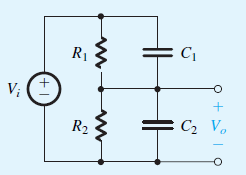
\includegraphics[scale=1.0]{P.1.80_enunciado.png}
\end{figure}

Sejam $Z_1 = R_1 \parallel C_1$ e $Z_2 = R_2 \parallel C_2$. Temos

\[ Z_1 = \frac{R_1\frac{1}{sC_1}}{R_1 + \frac{1}{sC_1}} = \frac{R_1}{sR_1C_1 + 1} \]

\[ Z_2 = \frac{R_2\frac{1}{sC_2}}{R_2 + \frac{1}{sC_2}} = \frac{R_2}{sR_2C_2 + 1} \]

Agora aplicamos a regra do divisor de tensão:

\[ V_o = V_i \frac{Z_2}{Z_1 + Z_2} \]

Substituindo e reorganizando os termos,

\[ V_o = V_i \frac{\frac{R_2}{sR_2C_2 + 1}}{\frac{R_1}{sR_1C_1 + 1} + \frac{R_2}{sR_2C_2 + 1}}  \]

\[ V_o = V_i \frac{\frac{R_2}{sR_2C_2 + 1}}{\frac{R_1(sR_2C_2 + 1) + R_2(sR_1C_1 + 1)}{(sR_1C_1 + 1)(sR_2C_2 + 1)}}  \]

\[ V_o = V_i \frac{R_2}{\frac{R_1(sR_2C_2 + 1) + R_2(sR_1C_1 + 1)}{sR_1C_1 + 1}}  \]

\[ \frac{V_o}{V_i} = \frac{R_2}{\frac{R_1(sR_2C_2 + 1)}{sR_1C_1 + 1} + R_2}  \]

\[ \frac{V_o}{V_i} = \frac{R_2}{\frac{sR_1R_2C_2 + R_1 + R_2(sR_1C_1 + 1)}{sR_1C_1 + 1}}  \]

\[ \frac{V_o}{V_i} = \frac{R_2(sR_1C_1 + 1)}{sR_1R_2C_2 + R_1 + R_2(sR_1C_1 + 1)}  \]

\[ \frac{V_o}{V_i} = \frac{sR_1R_2C_1 + R_2}{R_1 + R_2 + sR_1R_2C_2 + sR_2R_1C_1}  \]

\[ \frac{V_o}{V_i} = \frac{R_2 + sR_1R_2C_1}{R_1 + R_2 + s(R_1R_2C_2 + R_2R_1C_1)}  \]

Agora multiplicamos a fração pelo conjugado do denominador, lembrando que $s$ é uma variável complexa
dada por $s = j\omega$.

\[ \frac{V_o}{V_i} = \frac{(R_2 + sR_1R_2C_1) (R_1 + R_2 - s(R_1R_2C_2 + R_2R_1C_1))}{(R_1 + R_2)^2 + (R_1R_2C_2 + R_2R_1C_1)^2}  \]

Expandindo o produto no numerador através de distribuitiva, temos

\[ \frac{V_o}{V_i} = \frac{(R_1 + R_2)(sR_1R_2C_1) + R_2(R_1 + R_2) + (R_1R_2C_1)(R_1R_2C_2 + R_2R_1C_1) - sR_2(R_1R_2C_2 + R_2R_1C_1)}{(R_1 + R_2)^2 + (R_1R_2C_2 + R_2R_1C_1)^2}  \]

Colocando a parte imaginária em evidência no numerador,

\[ s\left[(R_1 + R_2)(R_1R_2C_1) - R_2(R_1R_2C_2 + R_2R_1C_1)\right] \]

A parte imaginária tem que ser nula para que a função de transferência não dependa
da frequência. Portanto,

\[ (R_1 + R_2)(R_1R_2C_1) - R_2(R_1R_2C_2 + R_2R_1C_1) = 0 \]

\[ (R_1 + R_2)(R_1R_2C_1) = R_2(R_1R_2C_2 + R_2R_1C_1) \]

\[ R_1^2R_2C_1 + R_1R_2^2C_1 = R_1R_2^2C_2 + R_1R_2^2C_1 \]

\[ R_1^2R_2C_1 = R_1R_2^2C_2 \]

\[ \boxed{ R_1C_1 = R_2C_2} \]

Finalmente, para que a função de transferência não dependa da frequência, temos que a condição 
$R_1C_1 = R_2C_2$ deve ser atendida, uma vez que a parte imaginária é nula nessa condição.\\

A análise com LTSpice desse problema está disponível no próximo arquivo em anexo.


\end{document}